\section{Algorithims}
\label{sec:Algorithims}

The novel hardware allows each M-Block module to identify their neighbors, even in the case of electrical failure of the
neighbor. This allows several algorithims...

%%% Overview figure...

This section gives a brief overview of three algorithms that are implemented on the robots. The results from these algorthms can be found in Section...
System overview
This section describes two different algorithms... These algorithms are similar to those described in...

%%%%%%%%%%%%%%%%%%%%%%%%%%%%%%%%%%%%%%%%%%%%%%%%%%%%%%%%%%%%%%%%%%%%%%%%%%%%%%%%%%%%%%%%%%%%%%%%%%%%%%%%%%%%%%%%%%%%%%%%%%%%%%%%%%%%%%%%%%%%%%%
%%%%%%%%%%%%%%%%%%%%%%%%%%%%%%%%%%%%%%%%%%%%%%%%%%%%%%%%%%%%%%%%%%%%%%%%%%%%%%%%%%%%%%%%%%%%%%%%%%%%%%%%%%%%%%%%%%%%%%%%%%%%%%%%%%%%%%%%%%%%%%%
\subsection{Arrow Following Algorithm}
\label{sec:algArrow}
%%%%%%%%%%%%%%%%%%%%%%%%%%%%%%%%%%%%%%%%%%%%%%%%%%%%%%%%%%%%%%%%%%%%%%%%%%%%%%%%%%%%%%%%%%%%%%%%%%%%%%%%%%%%%%%%%%%%%%%%%%%%%%%%%%%%%%%%%%%%%%%
%%%%%%%%%%%%%%%%%%%%%%%%%%%%%%%%%%%%%%%%%%%%%%%%%%%%%%%%%%%%%%%%%%%%%%%%%%%%%%%%%%%%%%%%%%%%%%%%%%%%%%%%%%%%%%%%%%%%%%%%%%%%%%%%%%%%%%%%%%%%%%%
% Three counters

%\begin{figure}[htb]  
  \centering

  \begin{subfigure}[b]{.3\linewidth}


    \resizebox{1 in}{0.6 in}
    {	\begin{tikzpicture}[x=(220:1cm), y=(-40:1cm), z=(90:0.707cm)]
    	


% Three counters
\newcounter{x}
\newcounter{y}
\newcounter{z}

% The angles of x,y,z-axes
\newcommand\xaxis{210}
\newcommand\yaxis{-30}
\newcommand\zaxis{90}

% The top side of a cube
\newcommand\topside[3]{
	\fill[fill=yellow, draw=black,shift={(\xaxis:#1)},shift={(\yaxis:#2)},
	shift={(\zaxis:#3)}] (0,0) -- (30:1) -- (0,1) --(150:1)--(0,0);
}

% The left side of a cube
\newcommand\leftside[3]{
	\fill[fill=red, draw=black,shift={(\xaxis:#1)},shift={(\yaxis:#2)},
	shift={(\zaxis:#3)}] (0,0) -- (0,-1) -- (210:1) --(150:1)--(0,0);
}

% The right side of a cube
\newcommand\rightside[3]{
	\fill[fill=blue, draw=black,shift={(\xaxis:#1)},shift={(\yaxis:#2)},
	shift={(\zaxis:#3)}] (0,0) -- (30:1) -- (-30:1) --(0,-1)--(0,0);
}

% The cube 
\newcommand\cube[3]{
	\topside{#1}{#2}{#3} \leftside{#1}{#2}{#3} \rightside{#1}{#2}{#3}
}

\newcommand\ArrowNE[3]
{
	\node at (#1+0.5, #2+0.5, #3) 
	{
		\begin{tikzpicture}
		\draw[->, thick, >={Stealth[round]}, line width=0.4mm] (0.3,0) -- (-0.3,0);
		\end{tikzpicture}};
		
}

\newcommand\ArrowNW[3]
{
	\node at (#1+0.5, #2+0.5, #3) 
	{
		\begin{tikzpicture}
		\draw[->, thick, >={Stealth[round]}, line width=0.4mm] (0,0.3) -- (0,-0.3);
		\end{tikzpicture}};
	
}

\newcommand\ArrowSW[3]
{
	\node at (#1+0.5, #2+0.5, #3) 
	{
		\begin{tikzpicture}
		\draw[<-, thick, >={Stealth[round]}, line width=0.4mm] (0.3,0) -- (-0.3,0);
		\end{tikzpicture}};
	
}

\newcommand\ArrowSE[3]
{
	\node at (#1+0.5, #2+0.5, #3) 
	{
		\begin{tikzpicture}
		\draw[<-, thick, >={Stealth[round]}, line width=0.4mm] (0,0.3) -- (0,-0.3);
		\end{tikzpicture}};
	
}

% Definition of \planepartition
% To draw the following plane partition, just write \planepartition{ {a, b, c}, {d,e} }.
%  a b c
%  d e
\newcommand\planepartition[1]{
	\setcounter{x}{-1}
	\foreach \a in {#1} {
		\addtocounter{x}{1}
		\setcounter{y}{-1}
		\foreach \b in \a {
			\addtocounter{y}{1}
			\setcounter{z}{-1}
			\foreach \c in {0,...,\b} {
				\addtocounter{z}{1}
				\ifthenelse{\c=0}{\setcounter{z}{-1},\addtocounter{y}{0}}{
					\cube{\value{x}}{\value{y}}{\value{z}}}
			}
		}
	}
}


\begin{tikzpicture}[x=(220:1cm), y=(-40:1cm), z=(90:0.707cm)]
	%\planepartition{{0,0,1},{1,1,1},{1,0,0},{1,0,1}};
\foreach \m [count=\y] in {{0,0,1},{1,1,1},{1,0,0},{1,0,0}}{
	\foreach \n [count=\x] in \m {
		\ifnum \n>0
		\foreach \z in {1,...,\n}{
			\draw [fill=blue!30] (\x+1,\y,\z) -- (\x+1,\y+1,\z) -- (\x+1, \y+1, \z-1) -- (\x+1, \y, \z-1) -- cycle;
			\draw [fill=blue!40] (\x,\y+1,\z) -- (\x+1,\y+1,\z) -- (\x+1, \y+1, \z-1) -- (\x, \y+1, \z-1) -- cycle;
			\draw [fill=blue!10] (\x,\y,\z)   -- (\x+1,\y,\z)   -- (\x+1, \y+1, \z)   -- (\x, \y+1, \z) -- cycle;  
		}
	
%		\node at (\x+0.5, \y+0.5, \n) 
%		{
%			\begin{tikzpicture}
%			\draw[->, thick, >={Stealth[round]}, line width=0.4mm] (-0.3,0) -- (0.3,0);
%			\end{tikzpicture}};
		
		\fi
	}
}   
\ArrowSW{2}{2}{1}
\ArrowNW{3}{2}{1}
\ArrowNW{3}{1}{1}
\ArrowSW{1}{2}{1}
\ArrowNW{1}{3}{1}
\ArrowNW{1}{4}{1}
%\drawArrow{1}{2}{1}
%\node at (2+0.5, 2+0.5, 1) 
%{
%	\begin{tikzpicture}
%	\draw[->, thick, >={Stealth[round]}, line width=0.4mm] (-0.3,0) -- (0.3,0);
%	\end{tikzpicture}};
%
%\node at (1+0.5, 2+0.5, 1) 
%{
%	\begin{tikzpicture}
%	\draw[->, thick, >={Stealth[round]}, line width=0.4mm] (0,0.3) -- (0,-0.3);
%	\end{tikzpicture}};`

\end{tikzpicture}
    	\ArrowSW{2}{2}{1}
    	\ArrowNW{3}{2}{1}
    	\ArrowNW{3}{1}{1}
    	\ArrowSW{1}{2}{1}
    	\ArrowNW{1}{3}{1}
    	\ArrowNW{1}{4}{1}
    	\end{tikzpicture}
    	
    }

    \subcaption{X-axis} 
  \end{subfigure}
  ~
  \begin{subfigure}[b]{.3\linewidth}

    \resizebox{1 in}{0.6 in}
    {
    {	\begin{tikzpicture}[x=(220:1cm), y=(-40:1cm), z=(90:0.707cm)]
    	


% Three counters
\newcounter{x}
\newcounter{y}
\newcounter{z}

% The angles of x,y,z-axes
\newcommand\xaxis{210}
\newcommand\yaxis{-30}
\newcommand\zaxis{90}

% The top side of a cube
\newcommand\topside[3]{
	\fill[fill=yellow, draw=black,shift={(\xaxis:#1)},shift={(\yaxis:#2)},
	shift={(\zaxis:#3)}] (0,0) -- (30:1) -- (0,1) --(150:1)--(0,0);
}

% The left side of a cube
\newcommand\leftside[3]{
	\fill[fill=red, draw=black,shift={(\xaxis:#1)},shift={(\yaxis:#2)},
	shift={(\zaxis:#3)}] (0,0) -- (0,-1) -- (210:1) --(150:1)--(0,0);
}

% The right side of a cube
\newcommand\rightside[3]{
	\fill[fill=blue, draw=black,shift={(\xaxis:#1)},shift={(\yaxis:#2)},
	shift={(\zaxis:#3)}] (0,0) -- (30:1) -- (-30:1) --(0,-1)--(0,0);
}

% The cube 
\newcommand\cube[3]{
	\topside{#1}{#2}{#3} \leftside{#1}{#2}{#3} \rightside{#1}{#2}{#3}
}

\newcommand\ArrowNE[3]
{
	\node at (#1+0.5, #2+0.5, #3) 
	{
		\begin{tikzpicture}
		\draw[->, thick, >={Stealth[round]}, line width=0.4mm] (0.3,0) -- (-0.3,0);
		\end{tikzpicture}};
		
}

\newcommand\ArrowNW[3]
{
	\node at (#1+0.5, #2+0.5, #3) 
	{
		\begin{tikzpicture}
		\draw[->, thick, >={Stealth[round]}, line width=0.4mm] (0,0.3) -- (0,-0.3);
		\end{tikzpicture}};
	
}

\newcommand\ArrowSW[3]
{
	\node at (#1+0.5, #2+0.5, #3) 
	{
		\begin{tikzpicture}
		\draw[<-, thick, >={Stealth[round]}, line width=0.4mm] (0.3,0) -- (-0.3,0);
		\end{tikzpicture}};
	
}

\newcommand\ArrowSE[3]
{
	\node at (#1+0.5, #2+0.5, #3) 
	{
		\begin{tikzpicture}
		\draw[<-, thick, >={Stealth[round]}, line width=0.4mm] (0,0.3) -- (0,-0.3);
		\end{tikzpicture}};
	
}

% Definition of \planepartition
% To draw the following plane partition, just write \planepartition{ {a, b, c}, {d,e} }.
%  a b c
%  d e
\newcommand\planepartition[1]{
	\setcounter{x}{-1}
	\foreach \a in {#1} {
		\addtocounter{x}{1}
		\setcounter{y}{-1}
		\foreach \b in \a {
			\addtocounter{y}{1}
			\setcounter{z}{-1}
			\foreach \c in {0,...,\b} {
				\addtocounter{z}{1}
				\ifthenelse{\c=0}{\setcounter{z}{-1},\addtocounter{y}{0}}{
					\cube{\value{x}}{\value{y}}{\value{z}}}
			}
		}
	}
}


\begin{tikzpicture}[x=(220:1cm), y=(-40:1cm), z=(90:0.707cm)]
	%\planepartition{{0,0,1},{1,1,1},{1,0,0},{1,0,1}};
\foreach \m [count=\y] in {{0,0,1},{1,1,1},{1,0,0},{1,0,0}}{
	\foreach \n [count=\x] in \m {
		\ifnum \n>0
		\foreach \z in {1,...,\n}{
			\draw [fill=blue!30] (\x+1,\y,\z) -- (\x+1,\y+1,\z) -- (\x+1, \y+1, \z-1) -- (\x+1, \y, \z-1) -- cycle;
			\draw [fill=blue!40] (\x,\y+1,\z) -- (\x+1,\y+1,\z) -- (\x+1, \y+1, \z-1) -- (\x, \y+1, \z-1) -- cycle;
			\draw [fill=blue!10] (\x,\y,\z)   -- (\x+1,\y,\z)   -- (\x+1, \y+1, \z)   -- (\x, \y+1, \z) -- cycle;  
		}
	
%		\node at (\x+0.5, \y+0.5, \n) 
%		{
%			\begin{tikzpicture}
%			\draw[->, thick, >={Stealth[round]}, line width=0.4mm] (-0.3,0) -- (0.3,0);
%			\end{tikzpicture}};
		
		\fi
	}
}   
\ArrowSW{2}{2}{1}
\ArrowNW{3}{2}{1}
\ArrowNW{3}{1}{1}
\ArrowSW{1}{2}{1}
\ArrowNW{1}{3}{1}
\ArrowNW{1}{4}{1}
%\drawArrow{1}{2}{1}
%\node at (2+0.5, 2+0.5, 1) 
%{
%	\begin{tikzpicture}
%	\draw[->, thick, >={Stealth[round]}, line width=0.4mm] (-0.3,0) -- (0.3,0);
%	\end{tikzpicture}};
%
%\node at (1+0.5, 2+0.5, 1) 
%{
%	\begin{tikzpicture}
%	\draw[->, thick, >={Stealth[round]}, line width=0.4mm] (0,0.3) -- (0,-0.3);
%	\end{tikzpicture}};`

\end{tikzpicture}
    	\ArrowSW{2}{2}{1}
    	\ArrowSW{3}{2}{1}
    	\ArrowSW{3}{1}{1}
    	\ArrowNE{1}{2}{1}
    	\ArrowNW{1}{3}{1}
    	\ArrowNW{1}{4}{1}
    	\end{tikzpicture}
    	
    }
	}

    \subcaption{Y-axis} 
  \end{subfigure}
  ~
  \begin{subfigure}[b]{.3\linewidth}
    \resizebox{1 in}{0.6 in}
    {
    	{	\begin{tikzpicture}[x=(220:1cm), y=(-40:1cm), z=(90:0.707cm)]
    		


% Three counters
\newcounter{x}
\newcounter{y}
\newcounter{z}

% The angles of x,y,z-axes
\newcommand\xaxis{210}
\newcommand\yaxis{-30}
\newcommand\zaxis{90}

% The top side of a cube
\newcommand\topside[3]{
	\fill[fill=yellow, draw=black,shift={(\xaxis:#1)},shift={(\yaxis:#2)},
	shift={(\zaxis:#3)}] (0,0) -- (30:1) -- (0,1) --(150:1)--(0,0);
}

% The left side of a cube
\newcommand\leftside[3]{
	\fill[fill=red, draw=black,shift={(\xaxis:#1)},shift={(\yaxis:#2)},
	shift={(\zaxis:#3)}] (0,0) -- (0,-1) -- (210:1) --(150:1)--(0,0);
}

% The right side of a cube
\newcommand\rightside[3]{
	\fill[fill=blue, draw=black,shift={(\xaxis:#1)},shift={(\yaxis:#2)},
	shift={(\zaxis:#3)}] (0,0) -- (30:1) -- (-30:1) --(0,-1)--(0,0);
}

% The cube 
\newcommand\cube[3]{
	\topside{#1}{#2}{#3} \leftside{#1}{#2}{#3} \rightside{#1}{#2}{#3}
}

\newcommand\ArrowNE[3]
{
	\node at (#1+0.5, #2+0.5, #3) 
	{
		\begin{tikzpicture}
		\draw[->, thick, >={Stealth[round]}, line width=0.4mm] (0.3,0) -- (-0.3,0);
		\end{tikzpicture}};
		
}

\newcommand\ArrowNW[3]
{
	\node at (#1+0.5, #2+0.5, #3) 
	{
		\begin{tikzpicture}
		\draw[->, thick, >={Stealth[round]}, line width=0.4mm] (0,0.3) -- (0,-0.3);
		\end{tikzpicture}};
	
}

\newcommand\ArrowSW[3]
{
	\node at (#1+0.5, #2+0.5, #3) 
	{
		\begin{tikzpicture}
		\draw[<-, thick, >={Stealth[round]}, line width=0.4mm] (0.3,0) -- (-0.3,0);
		\end{tikzpicture}};
	
}

\newcommand\ArrowSE[3]
{
	\node at (#1+0.5, #2+0.5, #3) 
	{
		\begin{tikzpicture}
		\draw[<-, thick, >={Stealth[round]}, line width=0.4mm] (0,0.3) -- (0,-0.3);
		\end{tikzpicture}};
	
}

% Definition of \planepartition
% To draw the following plane partition, just write \planepartition{ {a, b, c}, {d,e} }.
%  a b c
%  d e
\newcommand\planepartition[1]{
	\setcounter{x}{-1}
	\foreach \a in {#1} {
		\addtocounter{x}{1}
		\setcounter{y}{-1}
		\foreach \b in \a {
			\addtocounter{y}{1}
			\setcounter{z}{-1}
			\foreach \c in {0,...,\b} {
				\addtocounter{z}{1}
				\ifthenelse{\c=0}{\setcounter{z}{-1},\addtocounter{y}{0}}{
					\cube{\value{x}}{\value{y}}{\value{z}}}
			}
		}
	}
}


\begin{tikzpicture}[x=(220:1cm), y=(-40:1cm), z=(90:0.707cm)]
	%\planepartition{{0,0,1},{1,1,1},{1,0,0},{1,0,1}};
\foreach \m [count=\y] in {{0,0,1},{1,1,1},{1,0,0},{1,0,0}}{
	\foreach \n [count=\x] in \m {
		\ifnum \n>0
		\foreach \z in {1,...,\n}{
			\draw [fill=blue!30] (\x+1,\y,\z) -- (\x+1,\y+1,\z) -- (\x+1, \y+1, \z-1) -- (\x+1, \y, \z-1) -- cycle;
			\draw [fill=blue!40] (\x,\y+1,\z) -- (\x+1,\y+1,\z) -- (\x+1, \y+1, \z-1) -- (\x, \y+1, \z-1) -- cycle;
			\draw [fill=blue!10] (\x,\y,\z)   -- (\x+1,\y,\z)   -- (\x+1, \y+1, \z)   -- (\x, \y+1, \z) -- cycle;  
		}
	
%		\node at (\x+0.5, \y+0.5, \n) 
%		{
%			\begin{tikzpicture}
%			\draw[->, thick, >={Stealth[round]}, line width=0.4mm] (-0.3,0) -- (0.3,0);
%			\end{tikzpicture}};
		
		\fi
	}
}   
\ArrowSW{2}{2}{1}
\ArrowNW{3}{2}{1}
\ArrowNW{3}{1}{1}
\ArrowSW{1}{2}{1}
\ArrowNW{1}{3}{1}
\ArrowNW{1}{4}{1}
%\drawArrow{1}{2}{1}
%\node at (2+0.5, 2+0.5, 1) 
%{
%	\begin{tikzpicture}
%	\draw[->, thick, >={Stealth[round]}, line width=0.4mm] (-0.3,0) -- (0.3,0);
%	\end{tikzpicture}};
%
%\node at (1+0.5, 2+0.5, 1) 
%{
%	\begin{tikzpicture}
%	\draw[->, thick, >={Stealth[round]}, line width=0.4mm] (0,0.3) -- (0,-0.3);
%	\end{tikzpicture}};`

\end{tikzpicture}
    		\ArrowSW{2}{2}{1}
    		\ArrowSW{3}{2}{1}
    		\ArrowSW{3}{1}{1}
    		\ArrowSW{1}{2}{1}
    		\ArrowSW{1}{3}{1}
    		\ArrowSW{1}{4}{1}
    		\end{tikzpicture}
    		
    	}
    }
    \subcaption{Z-axis} 
  \end{subfigure}
%%  \subfloat[X-axis]{\includegraphics[width=1.1in]{Figures/FlywheelX.png}}
%%  \subfloat[Y-axis]{\includegraphics[width=1.1in]{Figures/FlywheelY.png}}
%%  \subfloat[Z-axis]{\includegraphics[width=1.1in]{Figures/FlywheelZ.png}}

\caption{The 3D M-Block changes the alignment of its flywheel by
	rotating the central assembly along a diagonal axis between two
	opposite corners of the frame (pointing out of the page).
	For every $2\pi/3$ radians of rotation along this axis, the
	flywheel comes into alignment with a new axis of the frame.}

\label{fig:PlaneChanging}    
\end{figure}
	
\begin{algorithm}[ht] 
	%\hrulefill
	\caption{Arrow Following Algorithm}
	\label{algorithmArrow}
	\SetAlgoLined
	\KwData{M-Blocks 3D}
	initialization\;
	\While{Connected to Valid module}
	{
		determine arrow direction\;
		\eIf{Plane is aligned}
		{
			Move in direction of arrow\;
		}
		{
			 Attempt to align flywheel with correct plane\;
		}
	}
	\caption{This algorithm attempts to drive a cube in the direction of the embedded direction defined by the \tagName on its neighbor cubes}

\end{algorithm}


%%%%%%%%%%%%%%%%%%%%%%%%%%%%%%%%%%%%%%%%%%%%%%%%%%%%%%%%%%%%%%%%%%%%%%%%%%%%%%%%%%%%%%%%%%%%%%%%%%%%%%%%%%%%%%%%%%%%%%%%%%%%%%%%%%%%%%%%%%%%%%%
%%%%%%%%%%%%%%%%%%%%%%%%%%%%%%%%%%%%%%%%%%%%%%%%%%%%%%%%%%%%%%%%%%%%%%%%%%%%%%%%%%%%%%%%%%%%%%%%%%%%%%%%%%%%%%%%%%%%%%%%%%%%%%%%%%%%%%%%%%%%%%%
\subsection{3D line formation algorithm}
\label{sec:algLine}
%%%%%%%%%%%%%%%%%%%%%%%%%%%%%%%%%%%%%%%%%%%%%%%%%%%%%%%%%%%%%%%%%%%%%%%%%%%%%%%%%%%%%%%%%%%%%%%%%%%%%%%%%%%%%%%%%%%%%%%%%%%%%%%%%%%%%%%%%%%%%%%
%%%%%%%%%%%%%%%%%%%%%%%%%%%%%%%%%%%%%%%%%%%%%%%%%%%%%%%%%%%%%%%%%%%%%%%%%%%%%%%%%%%%%%%%%%%%%%%%%%%%%%%%%%%%%%%%%%%%%%%%%%%%%%%%%%%%%%%%%%%%%%%
\subsection{Motion Planning - Arbitrary Shape to Line}
\label{ssec:line}
The goal of this experiment is to reconfigure an arbitrary 3D structure into a line. There are several approaches that could be applied to this, from implementing the full 3D algorithm described in ~\cite{sung2015reconfiguration}, to more simple approaches. These simple approaches could even be mostly distributed, for example, each module could check to see if it is part of the line (By asking through WIFI, or checking some local indicator, e.g. if the module it is attached to has its LED's turned on), and if not pick a direction and move that way. If it gets stuck, it could just detach from the structure and try to randomly attach back and try again.

\begin{figure}[h]  
	\centering
	\begin{subfigure}[b]{0.3\linewidth}
		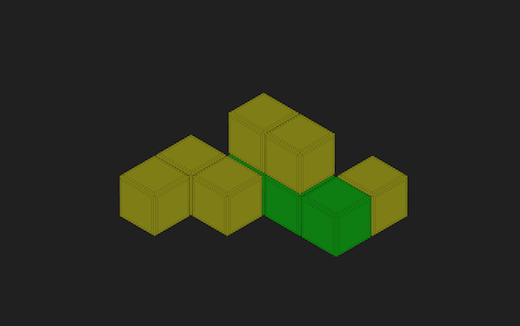
\includegraphics[width=0.9\linewidth]{figures/line_1.png}
		\subcaption{} 
	\end{subfigure}
	\begin{subfigure}[b]{0.3\linewidth}
		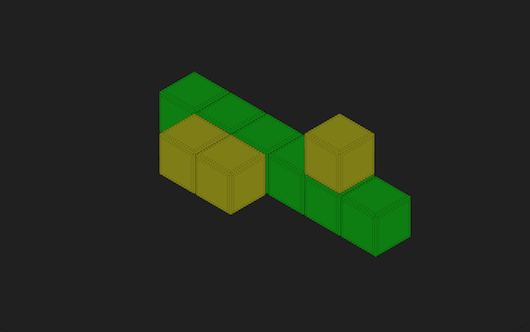
\includegraphics[width=0.9\linewidth]{figures/line_2.png}
		\subcaption{} 
	\end{subfigure}
	\begin{subfigure}[b]{0.3\linewidth}
		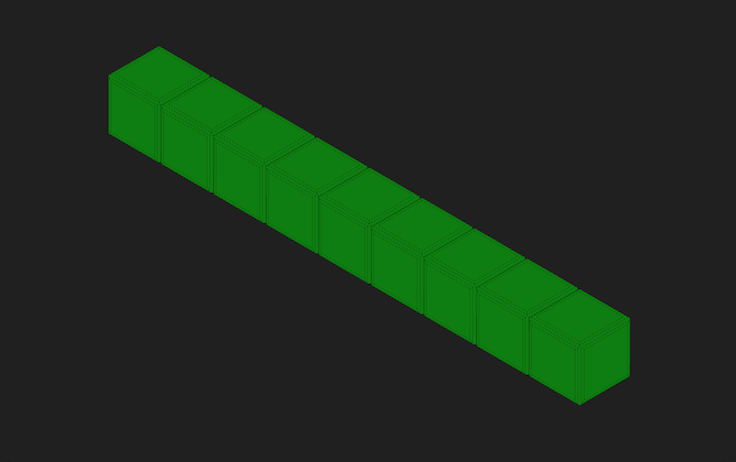
\includegraphics[width=0.9\linewidth]{figures/line_3.png}
		\subcaption{} 
	\end{subfigure}
	
	\caption{This experiment shows a random 3D configuration of M-Blocks reconfiguring into a line.}
	
	\label{fig:line}
\end{figure}

\begin{algorithm}[ht] 
	%\hrulefill
	\caption{Line formation Algorithm}
	\label{algorithmLine}
	\SetAlgoLined
	\KwData{M-Blocks 3D}
	initialization\;
	\While{Connected to Valid module}
	{
		determine arrow direction\;
		\eIf{Plane is aligned}
		{
			Move in direction of arrow\;
		}
		{
			Attempt to align flywheel with correct plane\;
		}
	}
	\caption{This algorithm attempts to drive }
	
\end{algorithm}


%%%%%%%%%%%%%%%%%%%%%%%%%%%%%%%%%%%%%%%%%%%%%%%%%%%%%%%%%%%%%%%%%%%%%%%%%%%%%%%%%%%%%%%%%%%%%%%%%%%%%%%%%%%%%%%%%%%%%%%%%%%%%%%%%%%%%%%%%%%%%%%
%%%%%%%%%%%%%%%%%%%%%%%%%%%%%%%%%%%%%%%%%%%%%%%%%%%%%%%%%%%%%%%%%%%%%%%%%%%%%%%%%%%%%%%%%%%%%%%%%%%%%%%%%%%%%%%%%%%%%%%%%%%%%%%%%%%%%%%%%%%%%%%
\subsection{Light Gradient based aggregation Algorithm}
\label{sec:algLight}
%%%%%%%%%%%%%%%%%%%%%%%%%%%%%%%%%%%%%%%%%%%%%%%%%%%%%%%%%%%%%%%%%%%%%%%%%%%%%%%%%%%%%%%%%%%%%%%%%%%%%%%%%%%%%%%%%%%%%%%%%%%%%%%%%%%%%%%%%%%%%%%
%%%%%%%%%%%%%%%%%%%%%%%%%%%%%%%%%%%%%%%%%%%%%%%%%%%%%%%%%%%%%%%%%%%%%%%%%%%%%%%%%%%%%%%%%%%%%%%%%%%%%%%%%%%%%%%%%%%%%%%%%%%%%%%%%%%%%%%%%%%%%%%
The goal of this experiment is to aggregate a group of modules nearby a light source to form one assembly. Placing the light source in a corner, and providing a \emph{seed} module can help to simplify aggregation, since the modules would know when to stop (When they see the seed module, or connect to a different module that has previously seen the seed module). One possible biological inspiration for this experiment is to imagine that the modules are cells of a plant, and the algorithm is to grow a structure towards the light source as a plant. As far as I know this work would be the first to accomplish this task in 3 dimensions using modular robots.

\begin{figure}[h]  
	\centering
	
	\begin{subfigure}[b]{0.3\linewidth}
		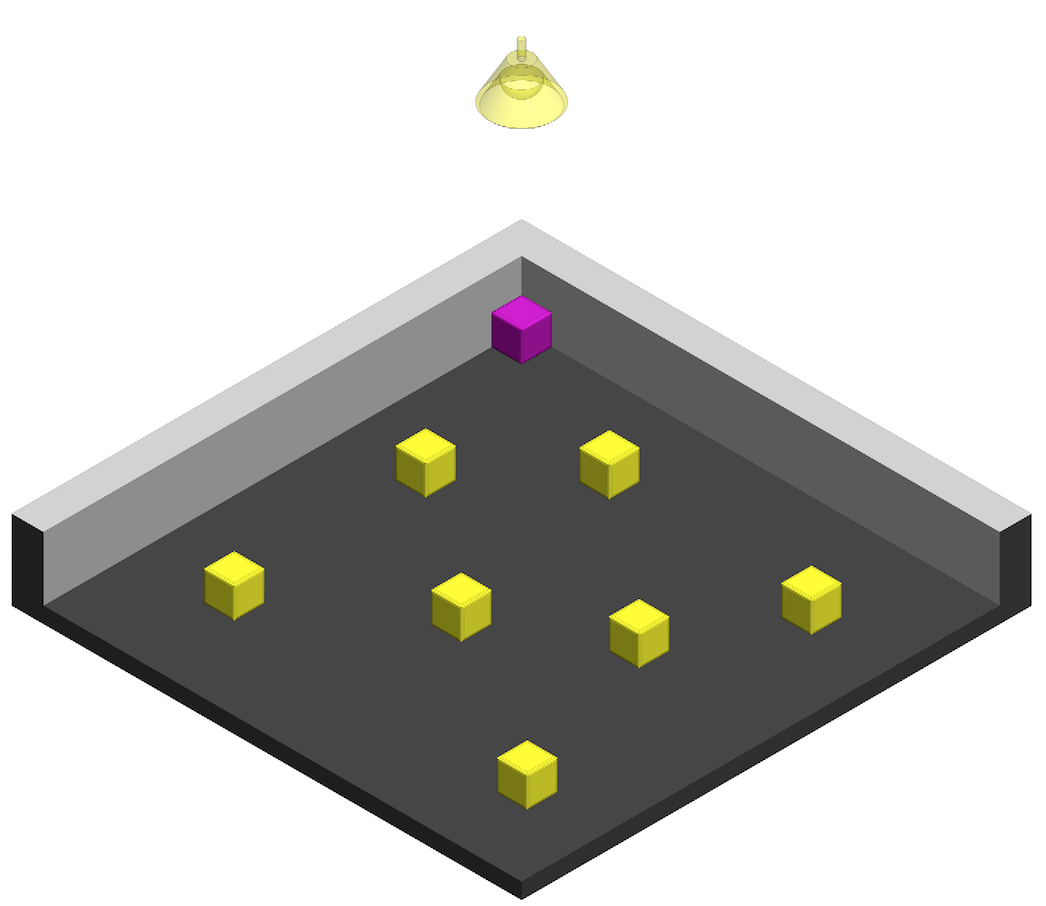
\includegraphics[width=0.9\linewidth]{figures/light_1.png}
		\subcaption{} 
	\end{subfigure}
	\begin{subfigure}[b]{0.3\linewidth}
		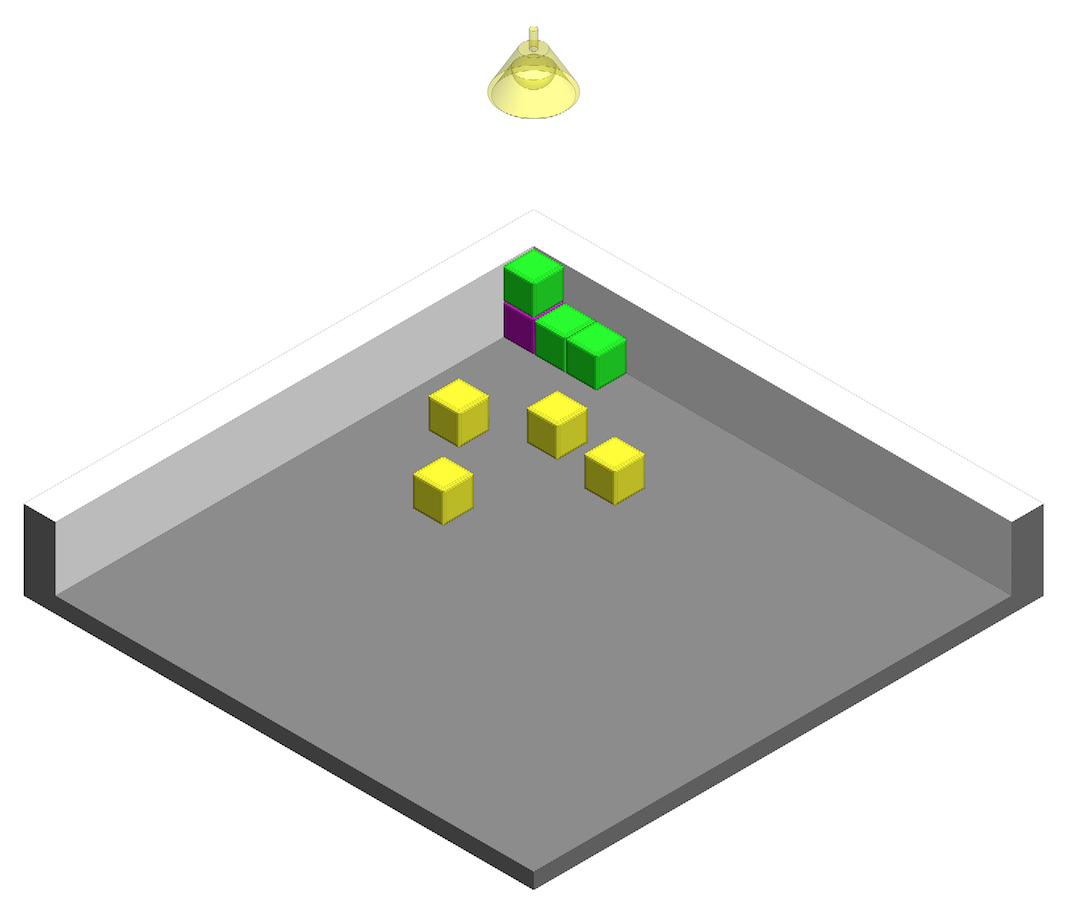
\includegraphics[width=0.9\linewidth]{figures/light_2.png}
		\subcaption{} 
	\end{subfigure}
	\begin{subfigure}[b]{0.3\linewidth}
		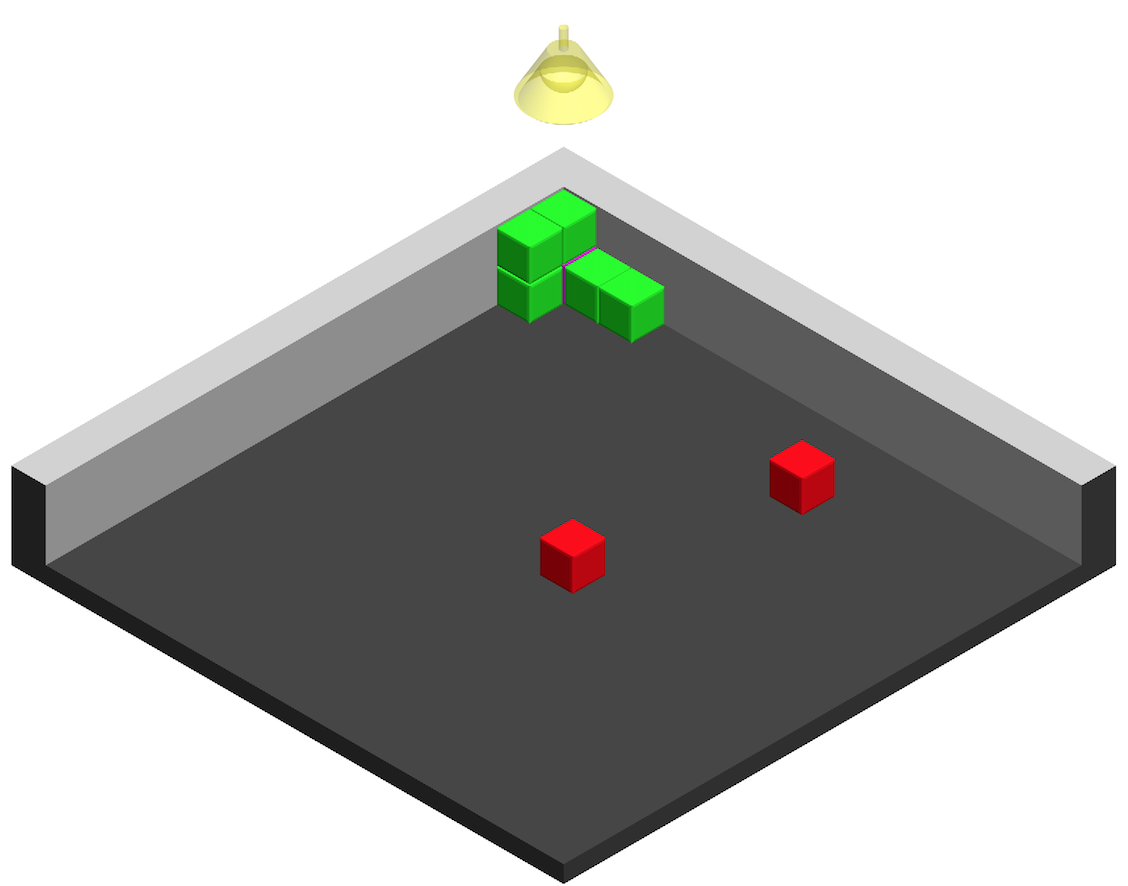
\includegraphics[width=0.9\linewidth]{figures/light_3.png}
		\subcaption{} 
	\end{subfigure}
	
	\caption{Three frames from an a illustration of the light-seeking experiment. One seed cube \emph{purple} is placed near the light, and the cubes in \emph{yellow} attempt to move towards the light. In the final frame, the modules which are in \emph{green} successfully reached the goal, while modules that are \emph{red} did not manage to join the target structure.}
	
	\label{fig:light}
\end{figure}

\textbf{Light Tracking Current Status}
\begin{itemize}
	\item Completely distributed software which can accomplish this task is already complete and running on the modules.
	\item Code to guide smaller aggregations that aren't at the target is completed, but still has lots of room for optimization.
\end{itemize}


\begin{algorithm}[htbp] 
	%\hrulefill
	\caption{Light guided aggregation Algorithm}
	\label{algorithmAggregate}
	\SetAlgoLined
	\KwData{M-Blocks 3D}
	initialization\;
	\While{Connected to Valid module}
	{
		determine arrow direction\;
		\eIf{Plane is aligned}
		{
			Move in direction of arrow\;
		}
		{
			Attempt to align flywheel with correct plane\;
		}
	}
	\caption{This algorithm attempts to drive a cube in the direction of the embedded direction defined by the \tagName on its neighbor cubes}
	
\end{algorithm}